\section{Real-World Case Study: Weak Supervision} \label{sec:exp}
\vspace{-.5em}
% We evaluate our theoretical findings and our proposed criterion. We anticipate that the value of data is significantly affected by misspecification, so that labeled data offers an insignificant value versus unlabeled (i.e., a small value ratio) for a well-specified model, but becomes more valuable as the misspecification level increases. We hypothesize that combining both labeled and unlabeled data can offer a superior estimate (as compared to relying one or the other alone). Finally, we expect that the bias due to misspecification is reflected downstream for a variety of models. 

% \subsection{Synthetic Data}

% \paragraph{Protocol}

% Our synthetic data distributions have balanced classes (i.e., $\mathbb{E}[Y]=0$) and $m=10$ labeling functions, with accuracies drawn uniformly from $[0.55, 0.75]$. Dependency strengths are fixed at $\varepsilon_{ij}=0.1$. To measure the expected generalization error of each learning algorithm for a given budget $n$, we perform $1000$ trials and average results, drawing data independently for each trial.

% {\color{red} Combination table goes here. Shows four columns: all labeled, all unlabeled, naive combination, and James-Stein.}


We validate our findings on real-world weak supervision dataset. We expect that some amount of misspecification is inevitable, and that this causes additional bias when learning from only unlabeled data. Unlike our theoretical setting where we limit the number of dependencies $d$ for simplicity, with real-world data we anticipate many small dependencies which cannot be completely corrected by the medians approach. We seek to answer the following key questions.

\begin{itemize}
    \item What is the standing parameter estimation bias due to misspecification? To what extent does the corrected estimator mitigate this bias?
    
    \item What is the data value ratio for the corrected estimator? %\steve{I like the other questions; maybe this question isn't necessary though? The standing bias means the labeled data ratio will depend on $n_U$} \bcw{I think I agree with the fact that the plot won't be very informative (it'll just be a line) but might be nice to have just to parallel the theoretical results.}
    
    \item Can a combined estimator with access to a small amount of labeled data provide substantial benefits over using only unlabeled data?
\end{itemize}
\vspace{-0.5em}

\paragraph{Protocol} Our real-world task is the sentiment analysis task of determining whether IMDB movie reviews are positive or negative \citep{maas2011learning}. The dataset contains 50K movie reviews, which we split into a training set of 40K reviews and a test set of 10K reviews. Our weak supervision sources are simple heuristics that vote ``yes'' when positive words appear and ``no'' when negative words appear. We provide further details in the Appendix.

% \steve{how did you pick the words? Especially the negative ones seem a little counterintuitive.} \bcw{I sorted words according to predictive power, and picked ones which seemed intuitive. I'm guessing you're referring to ``better'', ``could'' and ``would'' when you talk about the counterintuitive ones. These actually make sense to me, as they're referring to things like ``could have been better''} \steve{Can you add a few words describing the process then? Maybe: ``we chose words that were predictive and intuitive'' or something like that}

Unlike our theoretical model, where we assume that each source has a single accuracy parameter, we find that real-world sources have complex dependencies and can be better modeled with \textit{class conditional} accuracies. The method-of-moments approach in this setting results in a quadratic version of the triplet method \citep{fu2020fast}, the details of which we discuss in the Appendix. We use this version for our real-world case study, for which the same principles from our theoretical framework apply.
% We measure model performance in terms of its F1-score on the test set as a proxy for generalization error.
% For each dataset we train models with different label budgets $n_L$. We report the average accuracy on the test set over $1000$ trials (with different points to label selected for each trial). 

\vspace{-0.5em}
\paragraph{Standing bias and correction} For our first real-world experiment, we measure the standing parameter estimation bias when learning from unlabeled data (paralleling $\mathcal{B}_\text{est}$), and measure the decrease in  bias when using a corrected estimator. Recall that in our model a corrected estimator has an asymptotic estimation bias of $0$ given certain conditions on $d, m,$ and $n$. %when $d<\frac{(m-1)(m-2)}{4}$ for reasonable values of $m$ and $n$. 
On real data, however, we anticipate many small but complex dependencies that are not necessarily corrected for via our medians approach. 
%; $d$ might even be $m \choose 2$ but with most $\varepsilon_{ij}$ quite small.
Hence, we anticipate that the corrected estimator reduces $\mathcal{B}_\text{est}$ by mitigating the effects of larger dependencies while still being biased by the many small dependencies. We compute the test cross entropy loss for a labeled model, a baseline unlabeled and an unlabeled model with correction while varying $n$ and report results in \autoref{fig:real_biases_data_value_ratio}. Losses appear to converge, with a large gap between the labeled and unlabeled models and a smaller gap between the labeled model and the unlabeled model with correction. These gaps in loss are reflected by gaps in F1-scores, computed using a threshold of $.5$.

\begin{figure}
    \centering
    \begin{subfigure}{.48\textwidth}
      \centering
      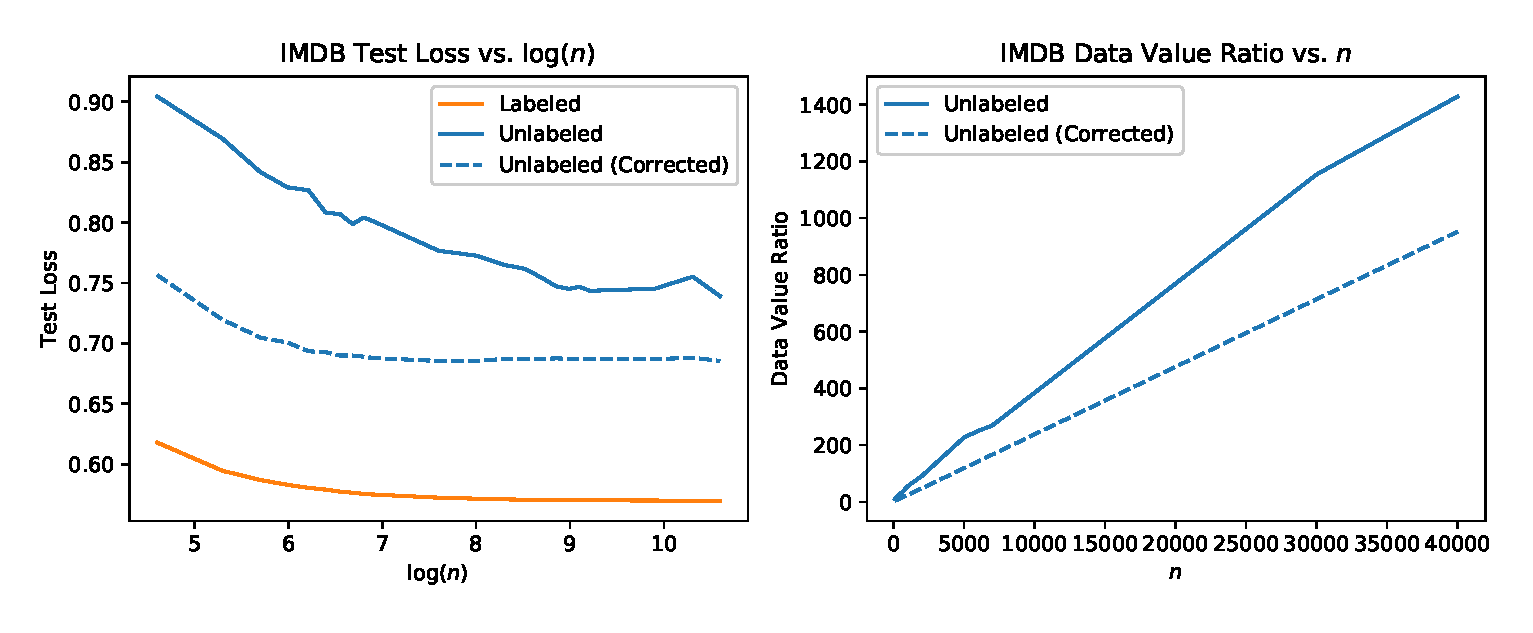
\includegraphics[width=\linewidth]{eps_figures/real_biases_data_value_ratio.eps}
    \end{subfigure}
   %
    \begin{subfigure}{.48\textwidth}
      \small
      \centering
      {\renewcommand{\arraystretch}{1.2}
      \begin{tabular}{lccr}
      \hline
      Model & Loss $(n=40\text{K})$ & F1 $(n=40\text{K})$ \\
      \hline
      Labeled & .570 & 71.79 \\
      Unlabeled & .740 & 64.81 \\
      Corrected & .686 & 68.12 \\
      \hline
      \end{tabular}
      }
    \end{subfigure}
    \caption{We measure test losses and F1-scores for labeled, unlabeled and corrected models on the IMDB dataset. Top Left: losses vs. $n$; each model appears to flatten out by $n=40,000$.  Bottom: losses and F1-scores at $n=40,000$, showing standing gaps in performance. Top Right: data value ratios for the two unlabeled models.}
    \label{fig:real_biases_data_value_ratio}
\end{figure}

\vspace{-0.5em}
\paragraph{Measuring the value of labeled data} Next, we measure the data value ratio in the real-world setting. Since both the unlabeled model and the unlabeled model with correction have a standing bias compared to the labeled model, we anticipate that the data value ratio for both unlabeled approaches grows linearly with $n$, with the data value ratio for the baseline unlabeled model having a greater constant factor due to its higher bias. We report these results in \autoref{fig:real_biases_data_value_ratio}.

% \begin{figure}
%     \centering
%     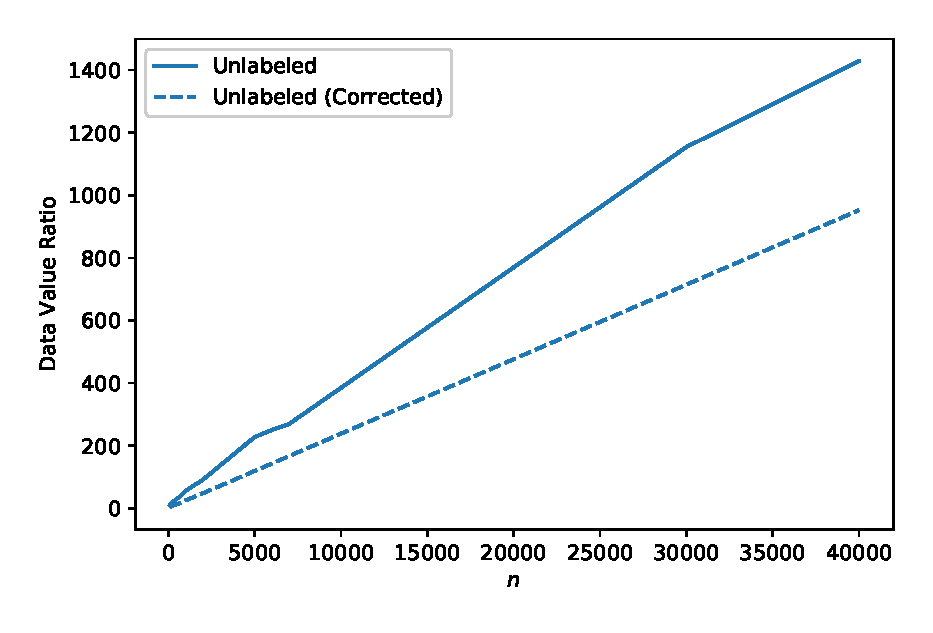
\includegraphics[width=.35\textwidth]{eps_figures/real_data_value_ratio.eps}
%    %
%     \caption{Data value ratio vs. $n$ for unlabeled and corrected models on the IMDB dataset. Both ratios increase linearly with $n$ because of the standing biases of the two unlabeled approaches; however, the ratio for the corrected model increases more slowly because its bias is smaller.}
%     \label{fig:real_data_value_ratio}
% \end{figure}

\vspace{-0.5em}
\paragraph{Combining labeled and unlabeled data} We finally measure the performance of the combined estimator from \cite{GreenStrawderman2001} in the setting where a small number of labeled points and many unlabeled points are available. We let $n_U=40,000$ be the entire training set and vary $n_L$ between $40$ and $400$. We use the corrected estimator for learning from unlabeled data. We report the F1-score using a threshold of $.5$. Results are in \autoref{tab:real_combo}. We observe that the combined estimator outperforms either approach individually for $n_L>40$.

% We use three tasks. First, \textbf{Spam} classification for Youtube comments ~\citep{alberto2015tubespam} has $10$ LFs from~\cite{Ratner19}. Here, the training set has $1586$ examples and the test set has $250$ examples; classes are approximately balanced. 

% In this case, we do not a priori know the level of misspecification. We expect that LFs are neither completely conditionally independent nor so markedly (conditionally) dependent that nothing can be learned from unlabeled data. This leads to data value ratios that are in between the scenarios in between the two extreme synthetic cases we considered above.

\begin{table}[t]
\vskip 0.15in
\renewcommand{\arraystretch}{1.25} % Default value: 1
\begin{center}
\begin{small}
\begin{tabular}{lccccr}
\hline
$n_U$ & $n_L$ & $\text{F1}_\text{Unlabeled}$ & $\text{F1}_\text{Labeled}$ &  $\text{F1}_\text{Combined}$ \\
\hline
40,000 & 40 & 68.12 & 64.70 & 67.06 \\
40,000 & 80 & 68.12 & 67.65 & 68.81 \\
40,000 & 120 & 68.12 & 68.92 & 69.64 \\
40,000 & 200 & 68.12 & 69.97 & 70.41 \\
40,000 & 400 & 68.12 & 70.81 & 71.04 \\
\hline
\end{tabular}
\end{small}
\end{center}
\vskip -0.1in
\caption{F1-scores for unlabeled, labeled and combined approaches on the IMDB dataset. We find that the combination generally outperforms either approach individually, and in particular both in cases where unlabeled only performs better and where labeled only performs better.}
\label{tab:real_combo}
\end{table}

% \begin{table}[t]
% \caption{F1-scores for weakly labeled, labeled and hybrid approaches over the \textbf{Spam} and \textbf{Spouse} datasets.}
% \label{sample-table}
% \vskip 0.15in
% \renewcommand{\arraystretch}{1.25} % Default value: 1
% \begin{center}
% \begin{small}
% \begin{tabular}{lcccccr}
% \hline
% \textbf{Task} & $n_U$ & $n_L$ & \bfseries{\scshape{FS}} & \bfseries{\scshape{MLE}} & \bfseries{\scshape{Comb.}} \\
% \hline
% Spam    & 1586 & 40 & 82.35 & 82.40 & 83.16 \\
% Spouse  & 3858 & 50 & 19.30 & 19.23 & 22.93 \\
% \hline
% \end{tabular}
% \end{small}
% \end{center}
% \vskip -0.1in
% \end{table}

% \begin{figure}
%     \centering
%     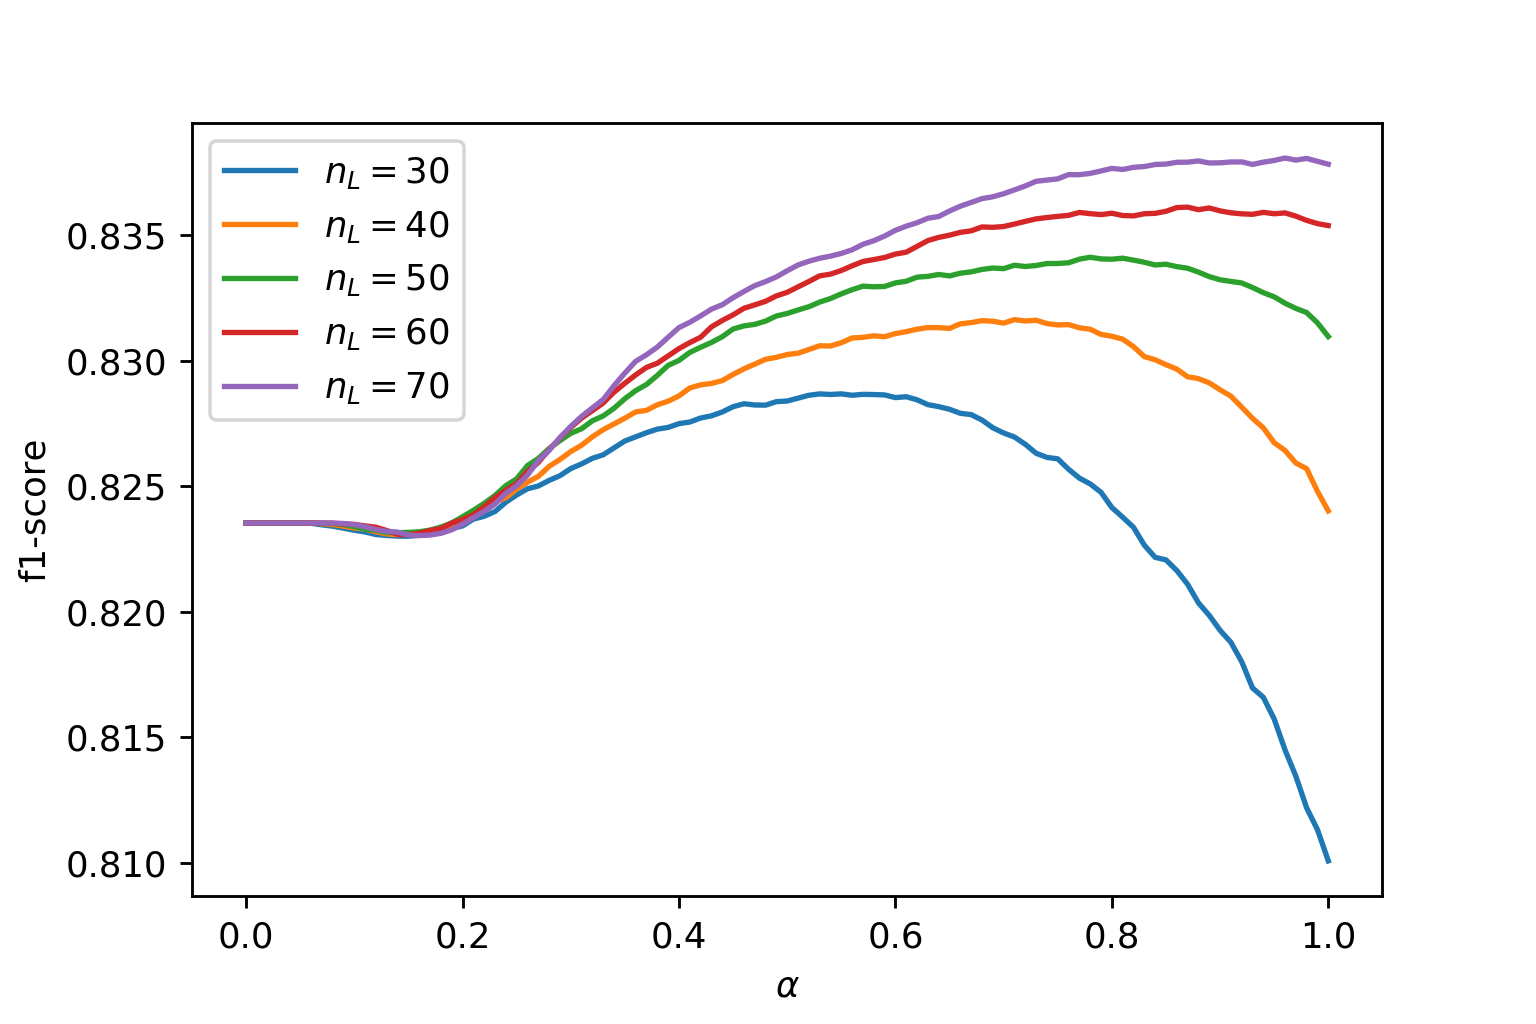
\includegraphics[width=.48\textwidth]{figures/spam_combined_estimator.png}
%     \caption{F1-score of a combined estimator varying combination weight $\alpha$ on the \textbf{Spam} dataset for different labeled budgets $n_L$ (the weakly labeled budget is the entire dataset). We see that combining labeled and weakly labeled approaches can outperform either individually.}
%     \label{fig:spam_combined_estimator}
% \end{figure}

% \subsection{Weak Labels, Standing Bias, and Downstream Models}
% Next, we measure the impact of bias in weak labels on end models trained on weak labels. We expect that when the weak labels do not have a standing bias, the generalization error is asymptotically identical to the case of training on fully-supervised labels. On the other hand, we hypothesize that biased weak labels will be reflected with a biased downstream model, no matter how much data we use, and that this bias is also a function of misspecification. That is, we expect that downstream models may not always be robust to weak labels.
% 
% \paragraph{Protocol}
% {\color{red} Gathering models for this step.}
% 
% \paragraph{Results}
% {\color{red} todo}

% \begin{figure}
%     \centering
%     \begin{minipage}{0.49\textwidth}
%         \centering
%         \includegraphics[width=0.9\textwidth]{figures/spam.pdf}
%         \caption{Accuracy for the \textbf{Spam} dataset with different budgets of labels and different unlabeled data weights $\gamma$.}
%         \label{fig:spam}
%     \end{minipage}\hfill
%     \begin{minipage}{0.49\textwidth}
%         \centering
%         \includegraphics[width=0.9\textwidth]{figures/amazon_reviews_1000.pdf}
%         \caption{Accuracy for the \textbf{Amazon Reviews} dataset with different budgets of labels and different unlabeled weights $\gamma$.}
%         \label{fig:amazon_reviews}
%     \end{minipage}
% \end{figure}
